\documentclass[12pt]{article}
\usepackage{amsthm,amssymb,amsfonts,amsmath,amstext,systeme}
\usepackage{graphicx,float}
\usepackage{tabularx}
\marginparwidth 0pt
\oddsidemargin -1.2 truecm
\evensidemargin  0pt 
\marginparsep 0pt
\topmargin -2.2truecm
\linespread{1}
\textheight 25.8 truecm
\textwidth 18.5 truecm
\newenvironment{remark}{\noindent{\bf Remark }}{\vspace{0mm}}
\newenvironment{remarks}{\noindent{\bf Remarks }}{\vspace{0mm}}
\newenvironment{question}{\noindent{\bf Question }}{\vspace{0mm}}
\newenvironment{questions}{\noindent{\bf Questions }}{\vspace{0mm}}
\newenvironment{note}{\noindent{\bf Note }}{\vspace{0mm}}
\newenvironment{summary}{\noindent{\bf Summary }}{\vspace{0mm}}
\newenvironment{back}{\noindent{\bf Background}}{\vspace{0mm}}
\newenvironment{conclude}{\noindent{\bf Conclusion}}{\vspace{0mm}}
\newenvironment{concludes}{\noindent{\bf Conclusions}}{\vspace{0mm}}
\newenvironment{dill}{\noindent{\bf Description of Dill's model}}{\vspace{0mm}}
\newenvironment{maths}{\noindent{\bf Mathematics needed}}{\vspace{0mm}}
\newenvironment{inst}{\noindent{\bf Instructions}}{\vspace{0mm}}
\newenvironment{notes}{\noindent{\bf Notes }}{\vspace{0mm}}
\newenvironment{theorem}{\noindent{\bf Theorem }}{\vspace{0mm}}
\newenvironment{example}{\noindent{\bf Example }}{\vspace{0mm}}
\newenvironment{examples}{\noindent{\bf Examples }}{\vspace{0mm}}
\newenvironment{topics}{\noindent{\bf Topics}}{\vspace{0mm}}
\newenvironment{outcomes}{\noindent{\bf Expected Learning Outcomes}}{\vspace{0mm}}
\newenvironment{lemma}{\noindent{\bf Lemma }}{\vspace{0mm}}
\newenvironment{solution}{\noindent{\it Solution}}{\vspace{2mm}}
\newcommand{\ds}{\displaystyle}
\newcommand{\un}{\underline}
\newcommand{\bs}{\boldsymbol}

\begin{document}

\baselineskip 18 pt
\begin{center}
	{\large \bf HKDSE MATH Core Practice Paper I}\\
	\vspace{2 mm}
\end{center}
\vspace{0.05cm}

\begin{enumerate}
	\item \textbf{HKDSE MATH Core Practice Paper I Q1}\\
	Simplify $\dfrac{(m^5n^{-2})^6}{m^4n^{-3}}$ and express your answer with positive indices. \\(3marks)

	\item \textbf{HKDSE MATH Core Practice Paper I Q2}\\
	Make $a$ the subject of the formula $\dfrac{5 + b}{1 - a} = 3b$. \\(3 marks)

	\item \textbf{HKDSE MATH Core Practice Paper I Q3}\\
	Factorize 
	\begin{enumerate}
		\item[(a)] $9x^2 - 42xy + 49y^2$,
		\item[(b)] $9x^2 - 42xy + 49y^2 - 6x + 14y$.
	\end{enumerate}
	(3 marks)

	\item \textbf{HKDSE MATH Core Practice Paper I Q4}\\
	The cost of a chair is \$360. If the chair is sold at a discount of 20\% on its marked price, then the percentage profit is 30\%. Find the marked price of the chair. \\(4 marks)
	
	\item \textbf{HKDSE MATH Core Practice Paper I Q5}\\
	The ratio of the capacity of a bottle to that of a cup is 4:3. The total capacity of 7 bottles and 9 cups is 11 litres. Find the capacity of a bottle. \\(4 marks)
	
	\item \textbf{HKDSE MATH Core Practice Paper I Q6}\\
	In a polar coordinate system, the polar coordinates of the points $A$, $B$ and $C$ are $(13, 157^\circ)$, $(14, 247^\circ)$ and $(15, 337^\circ)$ respectively.
	\begin{enumerate}
		\item[(a)] Let $O$ be the pole. Are $A$, $O$ and $C$ collinear? Explain your answer.
		\item[(b)] Find the area of $\triangle ABC$.
	\end{enumerate}
	(4 marks)

	\item \textbf{HKDSE MATH Core Practice Paper I Q7}\\
	In Figure 1, $BD$ is a diameter of the circle $ABCD$. If $AB = AC$ and $\angle BDC = 36^\circ$, find $\angle ABD$. \\(4 marks)
	\begin{figure}[H]
		\centering
		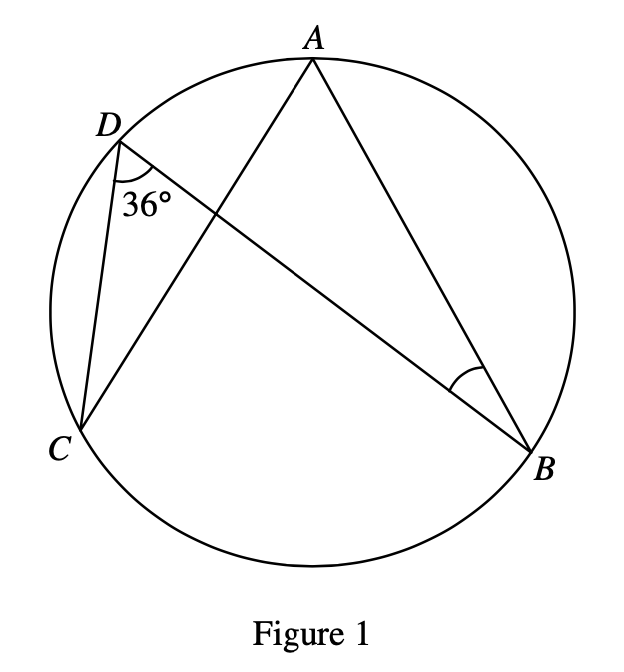
\includegraphics[width = .5\linewidth]{PPFigure1.1}
	\end{figure}

	\item \textbf{HKDSE MATH Core Practice Paper I Q8}\\
	The coordinates of the points $A$ and $B$ are $(-3,4)$ and $(-2, -5)$ respectively. $A'$ is the reflection image of $A$ with respect to the $y$-axis. $B$ is rotated anticlockwise about the origin $O$ through $90^\circ$ to $B'$.
	\begin{enumerate}
		\item[(a)] Write down the coordinates of $A'$ and $B'$.
		\item[(b)] Let $P$ be a moving point in the rectangular coordinate plane such that $P$ is equidistant from $A'$ and $B'$. Find the equation of the locus of $P$ .
	\end{enumerate}
	(5 marks)

	\item \textbf{HKDSE MATH Core Practice Paper I Q9}\\
	The following table shows the distribution of the numbers of online hours spent by a group of children
	on a certain day.
	$$\begin{array}{|l|c|c|c|c|}
		\hline
		\text{Number of online hours} & 2 & 3 & 4 & 5 \\
		\hline
		\text{Number of children} & r & 8 & 12 & s \\		
		\hline
	\end{array}$$
	It is given that $r$ and $s$ are positive numbers.
	\begin{enumerate}
		\item[(a)] Find the least possible value and the greatest possible value of the inter-quartile range of the distribution.
		\item[(b)] If $r = 9$ and the median of the distribution is 3, how many possible values of $s$ are there? Explain your answer.		
	\end{enumerate}
	(5 marks)

	\item \textbf{HKDSE MATH Core Practice Paper I Q10}\\
	Let $f(x)$ be a polynomial. When $f(x)$ is divided by $x - 1$ , the quotient is $6x^2 + 17x - 2$. It is given that $f(1) = 4$.
	\begin{enumerate}
		\item[(a)] Find $f(-3)$. \\(3 marks)
		\item[(b)] Factorize $f(x)$. \\(3 marks)
	\end{enumerate} 

	\item \textbf{HKDSE MATH Core Practice Paper I Q11}\\
	Let $\$ C$ be the cost of manufacturing a cubical carton of side $x$ cm. It is given that $C$ is partly constant and partly varies as the square of $x$. When $x = 20$, $C = 42$; when $x = 120$, $C = 112$.
	\begin{enumerate}
		\item Find the cost of manufacturing a cubical carton of side 50 cm. \\(4 marks)
		\item If the cost of manufacturing a cubical carton is \$58 , find the length of a side of the carton. \\(2 marks)
	\end{enumerate}

	\item \textbf{HKDSE MATH Core Practice Paper I Q12}\\
	Figure 2 shows the graphs for Ada and Billy running on the same straight road between town $P$ and town $Q$ during the period 1:00 to 3:00 in an afternoon. Ada runs at a constant speed. It is given that town $P$ and town $Q$ are 16 km apart.
	\begin{figure}[H]
		\centering
		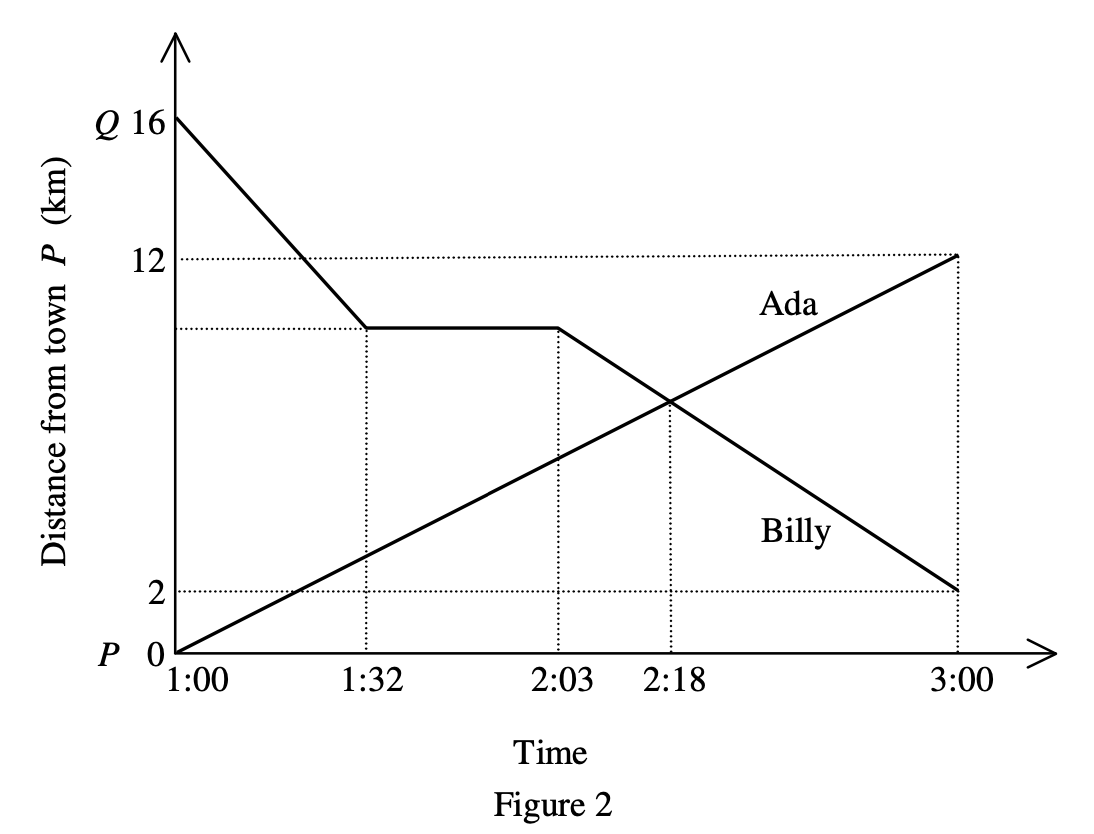
\includegraphics[width = .5\linewidth]{PPFigure1.2}
	\end{figure}
	\begin{enumerate}
		\item[(a)] How long does Billy rest during the period? \\(2 marks)
		\item[(b)] How far from town $P$ do Ada and Billy meet during the period? \\(3 marks)
		\item[(c)] Use average speed during the period to determine who runs faster. Explain your answer. \\(2 marks)
	\end{enumerate}

	\item \textbf{HKDSE MATH Core Practice Paper I Q13}\\
	The bar chart below shows the distribution of the most favourite fruits of the students in a group. It is given that each student has only one most favourite fruit.
	\begin{figure}[H]
		\centering
		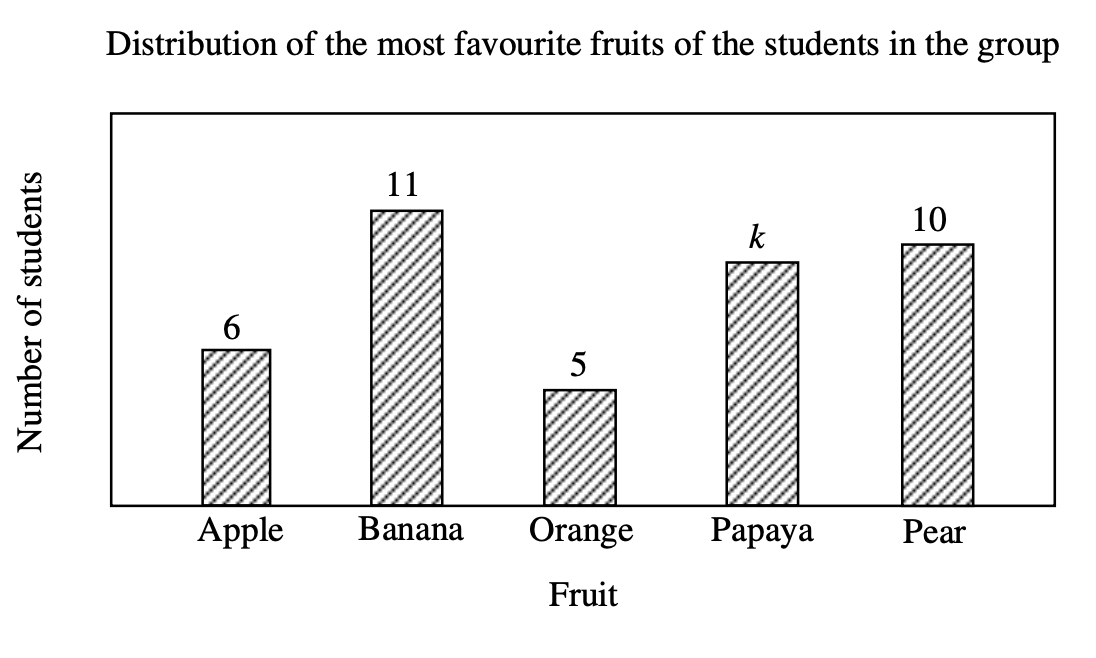
\includegraphics[width = .5\linewidth]{PPFigure1.00}
	\end{figure}
	If a student is randomly selected from the group, then the probability that the most favourite fruit is apple is $\dfrac{3}{20}$.
	\begin{enumerate}
		\item[(a)] Find $k$. \\(3 marks)
		\item[(b)] Suppose that the above distribution is represented by a pie chart.
		\begin{enumerate}
			\item[(ii)] Find the angle of the sector representing that the most favourite fruit is orange.
			\item[(i)] Some new students now join the group and the most favourite fruit of each of these students is orange. Will the angle of the sector representing that the most favourite fruit is orange be doubled? Explain your answer.
		\end{enumerate}
		(4 marks)
	\end{enumerate}

	\item \textbf{HKDSE MATH Core Practice Paper I Q14}\\
	In Figure 3, $OABC$ is a circle. It is given that $AB$ produced and $OC$ produced meet at $D$.
	\begin{figure}[H]
		\centering
		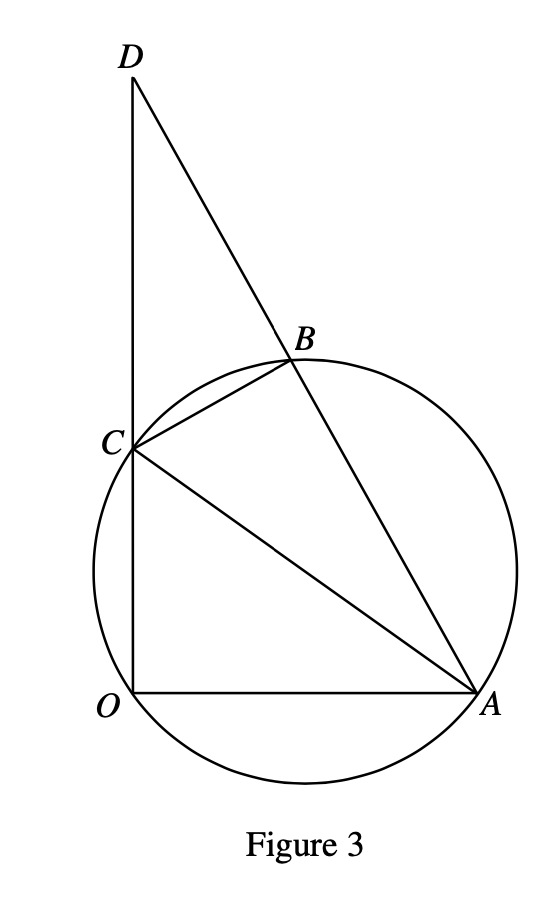
\includegraphics[width = .5\linewidth]{PPFigure1.3}
	\end{figure}
	\begin{enumerate}
		\item[(a)] Write down a pair of similar triangles in Figure 3. \\(2 marks)
		\item[(b)] Suppose that $\angle AOD = 90^\circ$. A rectangular coordinate system, with $O$ as the origin, is introduced in Figure 3 so that the coordinates of $A$ and $D$ are $(6,0)$ and $(0,12)$ respectively. If the ratio of the area of $\triangle BCD$ to the area of $\triangle OAD$ is 16:45, find
		\begin{enumerate}
			\item[(i)] the coordinates of $C$,
			\item[(ii)] the equation of the circle $OABC$.
		\end{enumerate}
		(7 marks)
	\end{enumerate}

	\item \textbf{HKDSE MATH Core Practice Paper I Q15}\\
	The mean score of a class of students in a test is 48 marks. The scores of Mary and John in the test are 36 marks and 66 marks respectively. The standard score of Mary in the test is $-2$.
	\begin{enumerate}
		\item[(a)] Find the standard score of John in the test. \\(2 marks)
		\item[(b)] A student, David, withdraws from the class and his test score is then deleted. It is given that his test score is 48 marks. Will there be any change in the standard score of John due to the deletion of the test score of David? Explain your answer. \\(2 marks)
	\end{enumerate}	


	\item \textbf{HKDSE MATH Core Practice Paper I Q16}\\
	There are 18 boys and 12 girls in a class. From the class, 4 students are randomly selected to form
	the class committee.
	\begin{enumerate}
		\item[(a)] Find the probability that the class committee consists of boys only. \\(2 marks)
		\item[(b)] Find the probability that the class committee consists of at least 1 boy and 1 girl. \\(2 marks)
	\end{enumerate}

	\item \textbf{HKDSE MATH Core Practice Paper I Q17}
	\begin{enumerate}
		\item[(a)] 	Express $\dfrac{1}{1 + 2i}$ in the form of $a + bi$, where $a$ and $b$ are real numbers. \\(2 marks)
		\item[(b)] The roots of the quadratic equation $x^2 + px + q = 0$ are $\dfrac{10}{1 + 2i}$ and $\dfrac{10}{1 - 2i}$. Find
		\begin{enumerate}
			\item[(i)] $p$ and $q$.
			\item[(ii)] the range of values of $r$ such that the quadratic equation $x^2 + px + q = r$ has real roots.
		\end{enumerate}
		(5 marks)
	\end{enumerate}

	\item \textbf{HKDSE MATH Core Practice Paper I Q18}\\
	Figure 4 shows a geometric model $ABCD$ in the form of tetrahedron. It is found that $\angle ACB = 60^\circ$,$AC = AD = 20$ cm, $BC = BD = 12$ cm and $CD = 14$ cm.
	\begin{figure}[H]
		\centering
		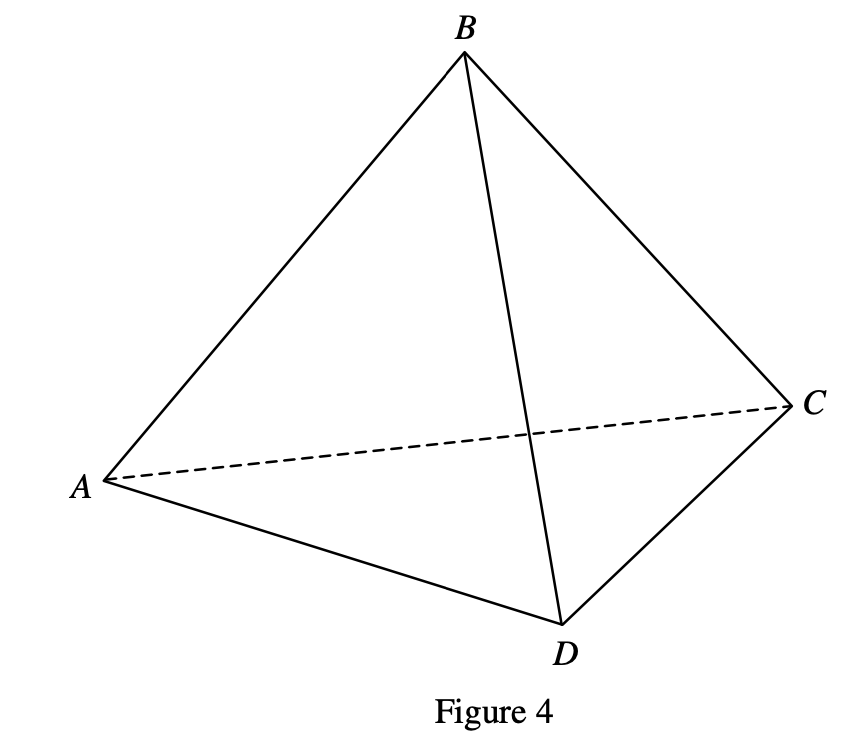
\includegraphics[width = .5\linewidth]{PPFigure1.4}
	\end{figure}
	\begin{enumerate}
		\item[(a)] Find the length of $AB$. \\(2 marks)
		\item[(b)] Find the angle between the plane $ABC$ and the plane $ABD$. \\(4 marks)
		\item[(c)] Let $P$ be a moving point on the slant edge $AB$. Describe how $\angle CPD$ varies as $P$ moves from $A$ to $B$. Explain your answer. \\(2 marks)
	\end{enumerate}

	\item \textbf{HKDSE MATH Core Practice Paper I Q19}\\
	The amount of investment of a commercial firm in the 1st year is \$4 000 000. The amount of investment in each successive year is $r \%$ less than the previous year. The amount of investment in the 4th year is \$1 048 576.
	\begin{enumerate}
		\item[(a)] Find $r$. \\(2 marks)
		\item[(b)] The revenue made by the firm in the 1st year is \$2 000 000. The revenue made in each successive year is 20\% less than the previous year.
		\begin{enumerate}
			\item[(i)] Find the least number of years needed for the total revenue made by the firm to exceed \$9 000 000.
			\item[(ii)] Will the total revenue made by the firm exceed \$10 000 000? Explain your answer.
			\item[(iii)] The manager of the firm claims that the total revenue made by the firm will exceed the total amount of investment. Do you agree? Explain your answer.	
		\end{enumerate}
		(10 marks)
	\end{enumerate}
\end{enumerate}
\end{document}

